% Original: PDF strana 19, donji slajd.
\slajdid{02-s038}
\begin{frame}[label=02-s038]{Karnoova karta za šest promenljivih}
\setlength{\parskip}{0pt}
% element: 02-s038:e01
\begin{columns}[T,onlytextwidth]
\begin{column}{.24\textwidth}\centering
\Oznaka{\(FE=00\)}\par\vspace{1mm}
\begingroup
\def\DEpomak{0}
% DC/BA: isti indeksi kao u izvornim kartama; DEpomak bira sloj FE.
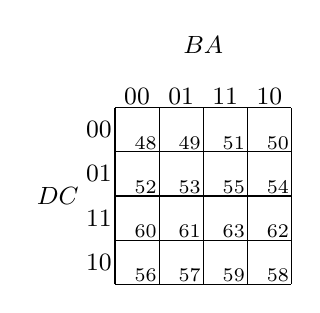
\begin{tikzpicture}[font=\fontsize{9}{10.5}\selectfont,x=5.6mm,y=5.6mm]
\draw[step=1,line width=.4pt] (0,0) grid (4,4);
\foreach \x/\lab in {.5/00,1.5/01,2.5/11,3.5/10}{\node[above,inner sep=1pt] at (\x,4) {\lab};}
\foreach \y/\lab in {3.5/00,2.5/01,1.5/11,.5/10}{\node[left,inner sep=1pt] at (0,\y) {\lab};}
\node[above] at (2,5) {\(BA\)};
\node[left] at (-.6,2) {\(DC\)};
\foreach \x/\y/\base in {.5/3.5/0,1.5/3.5/1,2.5/3.5/3,3.5/3.5/2,.5/2.5/4,1.5/2.5/5,2.5/2.5/7,3.5/2.5/6,.5/1.5/12,1.5/1.5/13,2.5/1.5/15,3.5/1.5/14,.5/.5/8,1.5/.5/9,2.5/.5/11,3.5/.5/10}{
 \pgfmathtruncatemacro{\indeks}{\base+\DEpomak}
 \node[anchor=south east,inner sep=.7pt,font=\fontsize{7}{8}\selectfont] at (\x+.5,\y-.5) {\indeks};
}
\end{tikzpicture}

\endgroup

\end{column}
\begin{column}{.24\textwidth}\centering
\Oznaka{\(FE=01\)}\par\vspace{1mm}
\begingroup
\def\DEpomak{16}
% DC/BA: isti indeksi kao u izvornim kartama; DEpomak bira sloj FE.
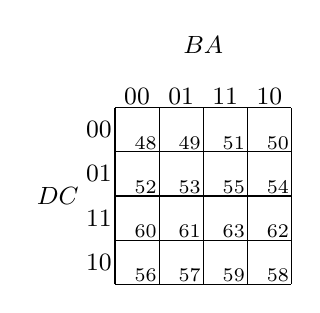
\begin{tikzpicture}[font=\fontsize{9}{10.5}\selectfont,x=5.6mm,y=5.6mm]
\draw[step=1,line width=.4pt] (0,0) grid (4,4);
\foreach \x/\lab in {.5/00,1.5/01,2.5/11,3.5/10}{\node[above,inner sep=1pt] at (\x,4) {\lab};}
\foreach \y/\lab in {3.5/00,2.5/01,1.5/11,.5/10}{\node[left,inner sep=1pt] at (0,\y) {\lab};}
\node[above] at (2,5) {\(BA\)};
\node[left] at (-.6,2) {\(DC\)};
\foreach \x/\y/\base in {.5/3.5/0,1.5/3.5/1,2.5/3.5/3,3.5/3.5/2,.5/2.5/4,1.5/2.5/5,2.5/2.5/7,3.5/2.5/6,.5/1.5/12,1.5/1.5/13,2.5/1.5/15,3.5/1.5/14,.5/.5/8,1.5/.5/9,2.5/.5/11,3.5/.5/10}{
 \pgfmathtruncatemacro{\indeks}{\base+\DEpomak}
 \node[anchor=south east,inner sep=.7pt,font=\fontsize{7}{8}\selectfont] at (\x+.5,\y-.5) {\indeks};
}
\end{tikzpicture}

\endgroup

\end{column}
\begin{column}{.24\textwidth}\centering
\Oznaka{\(FE=10\)}\par\vspace{1mm}
\begingroup
\def\DEpomak{32}
% DC/BA: isti indeksi kao u izvornim kartama; DEpomak bira sloj FE.
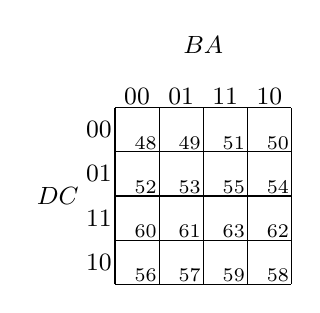
\begin{tikzpicture}[font=\fontsize{9}{10.5}\selectfont,x=5.6mm,y=5.6mm]
\draw[step=1,line width=.4pt] (0,0) grid (4,4);
\foreach \x/\lab in {.5/00,1.5/01,2.5/11,3.5/10}{\node[above,inner sep=1pt] at (\x,4) {\lab};}
\foreach \y/\lab in {3.5/00,2.5/01,1.5/11,.5/10}{\node[left,inner sep=1pt] at (0,\y) {\lab};}
\node[above] at (2,5) {\(BA\)};
\node[left] at (-.6,2) {\(DC\)};
\foreach \x/\y/\base in {.5/3.5/0,1.5/3.5/1,2.5/3.5/3,3.5/3.5/2,.5/2.5/4,1.5/2.5/5,2.5/2.5/7,3.5/2.5/6,.5/1.5/12,1.5/1.5/13,2.5/1.5/15,3.5/1.5/14,.5/.5/8,1.5/.5/9,2.5/.5/11,3.5/.5/10}{
 \pgfmathtruncatemacro{\indeks}{\base+\DEpomak}
 \node[anchor=south east,inner sep=.7pt,font=\fontsize{7}{8}\selectfont] at (\x+.5,\y-.5) {\indeks};
}
\end{tikzpicture}

\endgroup

\end{column}
\begin{column}{.24\textwidth}\centering
\Oznaka{\(FE=11\)}\par\vspace{1mm}
\begingroup
\def\DEpomak{48}
% DC/BA: isti indeksi kao u izvornim kartama; DEpomak bira sloj FE.
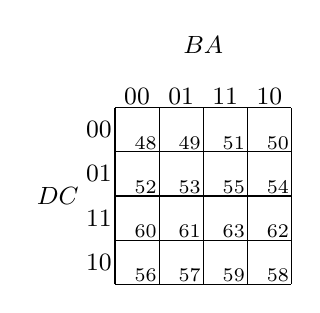
\begin{tikzpicture}[font=\fontsize{9}{10.5}\selectfont,x=5.6mm,y=5.6mm]
\draw[step=1,line width=.4pt] (0,0) grid (4,4);
\foreach \x/\lab in {.5/00,1.5/01,2.5/11,3.5/10}{\node[above,inner sep=1pt] at (\x,4) {\lab};}
\foreach \y/\lab in {3.5/00,2.5/01,1.5/11,.5/10}{\node[left,inner sep=1pt] at (0,\y) {\lab};}
\node[above] at (2,5) {\(BA\)};
\node[left] at (-.6,2) {\(DC\)};
\foreach \x/\y/\base in {.5/3.5/0,1.5/3.5/1,2.5/3.5/3,3.5/3.5/2,.5/2.5/4,1.5/2.5/5,2.5/2.5/7,3.5/2.5/6,.5/1.5/12,1.5/1.5/13,2.5/1.5/15,3.5/1.5/14,.5/.5/8,1.5/.5/9,2.5/.5/11,3.5/.5/10}{
 \pgfmathtruncatemacro{\indeks}{\base+\DEpomak}
 \node[anchor=south east,inner sep=.7pt,font=\fontsize{7}{8}\selectfont] at (\x+.5,\y-.5) {\indeks};
}
\end{tikzpicture}

\endgroup

\end{column}
\end{columns}
\par\vspace{3mm}
% element: 02-s038:e02
\Oznaka{Susedstvo između karata}
Pored susedstva unutar svake karte, u 4D prostoru susedna polja dobijamo i preklapanjem odgovarajućih karata: \(0\leftrightarrow32\), \(1\leftrightarrow33\), \(16\leftrightarrow48\), \(17\leftrightarrow49\), itd.
\end{frame}
